\section{Results and Discussions}
\label{sec:results}

\fablenote{Retitle to ``Results and Discussion'' (singular --- ``Discussions'' is non-standard). Structural suggestion for A+ readability: open the section with a 3-sentence summary paragraph stating the three headline findings before any table, so a skimming reviewer gets the verdict in 10 seconds. The single most valuable addition to this section is the commented-out Pareto-frontier figure above --- restore it (or a 2$\times$2 subset): a frontier plot where \textsc{VOILA}'s $\lambda$-sweep curve dominates every baseline point is the one figure that defuses the ``10 points below full resolution'' objection, because it shows VOILA at EVERY operating point, not one.}

% \begin{figure*}[htb]
%     \centering
%     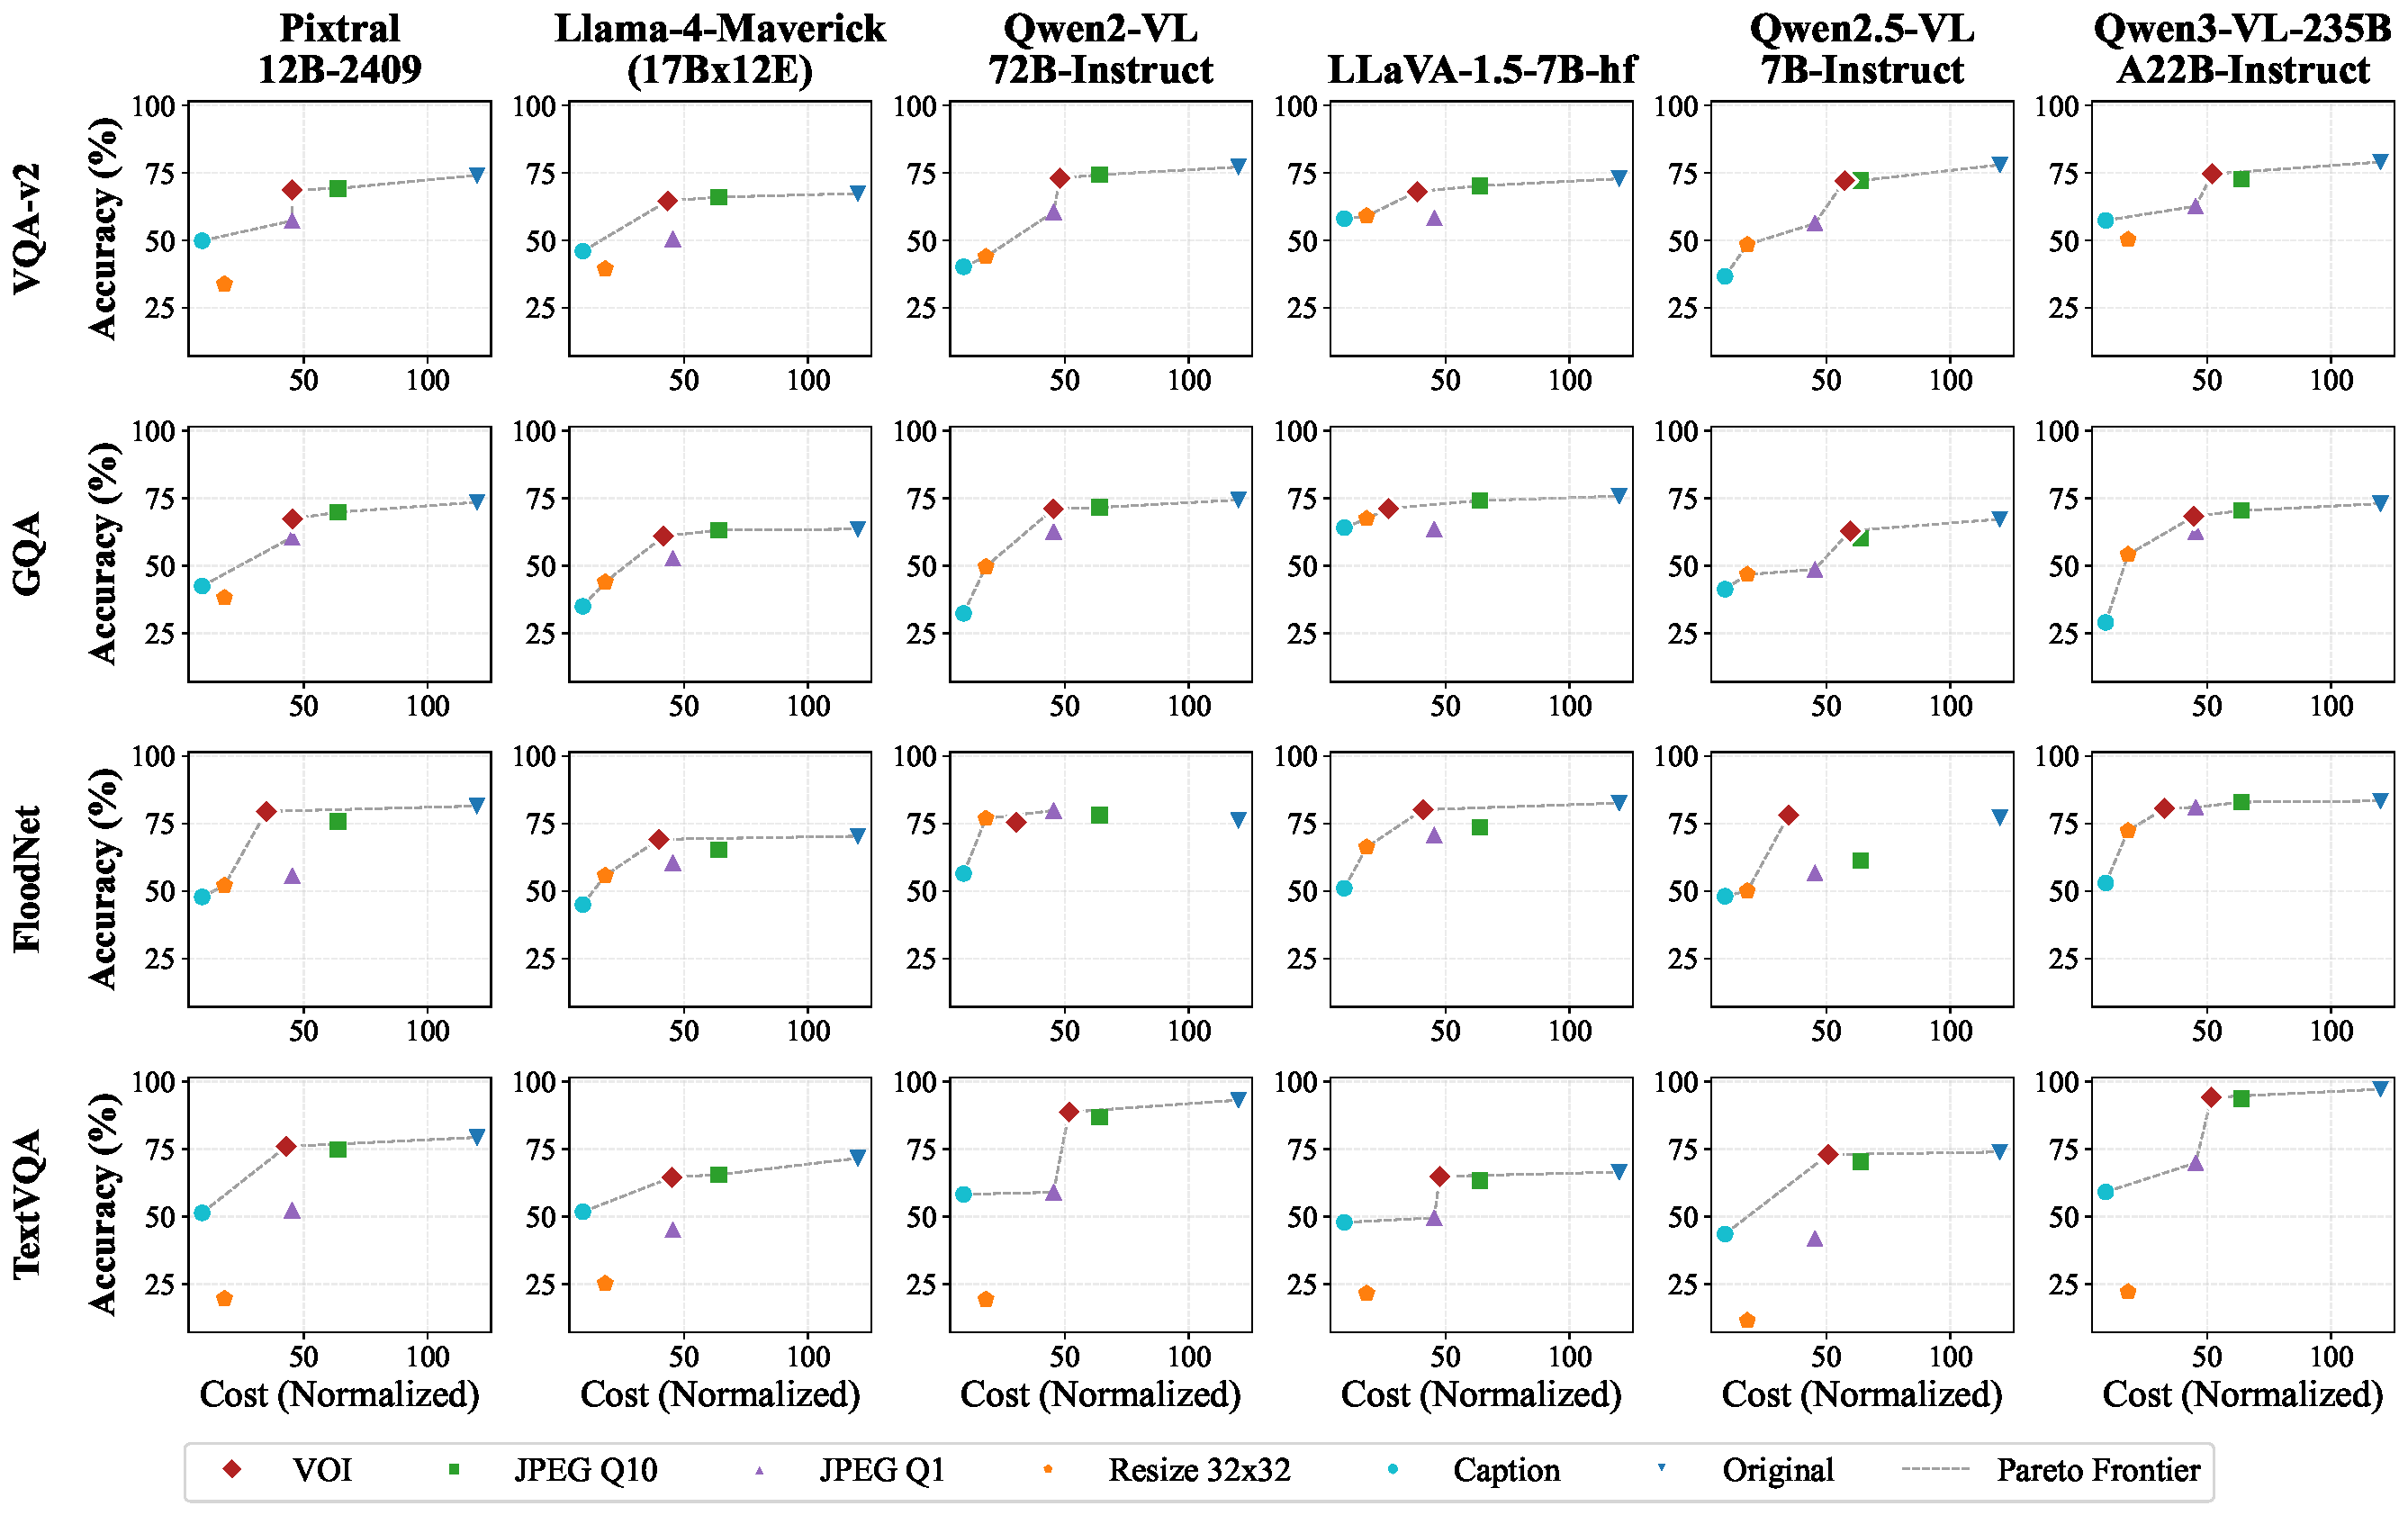
\includegraphics[width=0.95\linewidth]{plots/pareto_frontier_plot.pdf}
%     \caption{\textbf{Accuracy--cost Pareto frontiers across datasets and models.}
% Each subplot plots accuracy versus normalized retrieval cost (upper left is better) for a dataset--model pair, comparing \textsc{VOILA} to fixed-fidelity baselines, the Log-prob Cascade, the GPT-4o LLM Router, and the Oracle upper bound.
% Dashed curves denote Pareto frontiers.
% Across datasets and model scales, \textsc{VOILA} lies on or near the frontier, achieving near--full-resolution accuracy at 60--80\% lower average cost.}
%     \label{fig:pareto}
% \end{figure*}

\begin{table*}[htb]
\centering
\small
\setlength{\tabcolsep}{4pt}
\renewcommand{\arraystretch}{0.90}
\caption{\textbf{Average Acc\,(\%) and Cost across six VLMs} on four in-distribution benchmarks and LoCoMo$^\dagger$ (zero-shot OOD). Cost normalized so full-resolution $=100$; lower is better. \textsc{VOILA} rows bolded. Full per-VLM breakdown in Table~\ref{tab:complete_results} (Appendix~\ref{sec:complete_results}).}
\label{tab:master_comparison}
\resizebox{\linewidth}{!}{\begin{tabular}{@{}l rr rr rr rr rr@{}}
\toprule
& \multicolumn{2}{c}{\textbf{VQA-v2}}
& \multicolumn{2}{c}{\textbf{GQA}}
& \multicolumn{2}{c}{\textbf{TextVQA}}
& \multicolumn{2}{c}{\textbf{FloodNet}}
& \multicolumn{2}{c}{\textbf{LoCoMo}$^\dagger$} \\
\cmidrule(lr){2-3}\cmidrule(lr){4-5}\cmidrule(lr){6-7}\cmidrule(lr){8-9}\cmidrule(lr){10-11}
\textbf{Method} & Acc\% & Cost & Acc\% & Cost & Acc\% & Cost & Acc\% & Cost & Acc\% & Cost \\
\midrule
\multicolumn{11}{l}{\textit{Fixed fidelity}} \\[1pt]
Caption        & 47.8 & 7.6  & 39.9 & 7.6  & 75.7 & 7.6  & 41.8 & 7.6  & 29.6 & 7.6  \\
Full           & 75.0 & 100  & 70.2 & 100  & 86.6 & 100  & 60.1 & 100  & 59.8 & 100  \\
\midrule
\multicolumn{11}{l}{\textit{Adaptive baselines}} \\[1pt]
Log-prob Cascade   & 54.5 & 36.6 & 51.1 & 44.7 & 71.9 & 39.3 & 55.8 & 38.1 & 31.5 & 36.9 \\
GPT-4o Router      & 67.2 & 49.2 & 57.7 & 40.5 & 84.5 & 70.7 & 55.1 & 46.3 & 48.5 & 43.3 \\
BERT Router        & 62.0 & 40.9 & 59.7 & 40.9 & 71.9 & 33.1 & 59.8 & 39.2 & 47.2 & 51.8 \\
\textsc{VOILA}-CDF & 55.5 & 18.1 & 55.5 & 21.1 & 72.1 & 25.1 & 58.2 & 41.8 & \multicolumn{2}{c}{---} \\
\midrule
\multicolumn{11}{l}{\textit{Upper bound}} \\[1pt]
Oracle             & 86.9 & 29.8 & 83.5 & 33.2 & 96.7 & 18.2 & 81.5 & 35.6 & 79.0 & 41.9 \\
\midrule
\textbf{\textsc{VOILA} (ours)} & \textbf{64.9} & \textbf{35.2} & \textbf{59.6} & \textbf{27.9} & \textbf{84.8} & \textbf{26.6} & \textbf{63.5} & \textbf{19.3} & \textbf{45.1} & \textbf{36.6} \\
\bottomrule
\end{tabular}}
{\footnotesize $^\dagger$Zero-shot OOD (trained on VQA-v2+GQA); 2 VLMs only (Pixtral-12B, Qwen2.5-VL-7B). ``---'' = not evaluated.}
\end{table*}

\fablenote{Table~\ref{tab:master_comparison} issues to fix for AAAI: (1) On VQA-v2 the GPT-4o Router (67.2) beats \textsc{VOILA} (64.9) on raw accuracy --- the bolded VOILA row visually claims a win the numbers do not show. Add a matched-cost row (\textsc{VOILA} with $\lambda$ tuned to cost $\approx$49) or an accuracy-per-cost column so the table itself demonstrates dominance. (2) No variance: add bootstrap 95\% CIs or at least mark which gaps are significant. (3) The LoCoMo column averages 2 VLMs while others average 6 --- footnote this in the caption text, not only the dagger, or reviewers will catch the apples-to-oranges averaging. (4) Report the GPT-4o Router's own routing cost (one GPT-4o call per query is not free); currently its Cost column counts only retrieval, which flatters the baseline you beat and undersells your win.}

\textbf{VOILA consistently matches near-full-resolution accuracy at dramatically lower cost.}
Table~\ref{tab:master_comparison} reports per-VLM accuracy and cost for all methods across four datasets.
\textsc{VOILA} lies consistently close to the full-resolution operating point across all four datasets and all six VLMs, while operating at substantially lower retrieval cost.
Fidelity selection distributions are provided in Appendix~\ref{sec:complete_results} (Figure~\ref{fig:voila_fidelity_distribution}).
On VQA-v2, \textsc{VOILA} achieves an average accuracy of 64.9\% at an average cost of 35.1, compared to 75.0\% at cost 100 for full-resolution --- a gap of only 10.1 accuracy points while reducing retrieval cost by 65\%.
On TextVQA, the gap narrows to 1.8 accuracy points (84.8\% vs.\ 86.6\%) while reducing cost by 73\%, demonstrating that \textsc{VOILA} can almost exactly recover full-resolution performance at a fraction of the cost when caption-level text descriptions are sufficient for the dominant question types.
On FloodNet, \textsc{VOILA} (avg.\ 63.5\%) actually \emph{exceeds} fixed-cost full-resolution accuracy (avg.\ 60.1\%) while operating at less than 20\% of the full-resolution retrieval cost --- a result attributable to adaptive routing away from modalities where high-resolution imagery does not improve accuracy for this model and question distribution.
\fablenote{The first paragraph's numbers disagree with the table: text says cost 35.1 on VQA-v2, Table~\ref{tab:master_comparison} says 35.2; text says TextVQA gap 1.8 points but 86.6$-$84.8$=$1.8 at 73\% cost reduction while the table cost (26.6) implies 73.4\%. Sweep every inline number against the table before submission --- AAAI reviewers spot-check these. Also, ``adaptive routing away from modalities'' is the wrong word (fidelities, not modalities).}
Per-question-type analysis reveals the mechanism: Condition Recognition queries---the dominant FloodNet category---consistently peak at compressed fidelities across most models (e.g., Pixtral-12B at JPEG Q10: 61.9\%; LLaVA-1.5-7B at caption: 91.3\%; Qwen2-VL-72B at $32{\times}32$ resize: 98.8\%; Qwen3-VL-235B at JPEG Q1: 98.0\%), while counting queries require full resolution.
\textsc{VOILA} routes Condition Recognition queries to their optimal compressed fidelity and counting queries to full resolution, achieving higher average accuracy than the full-resolution baseline, which incurs unnecessary bandwidth cost on Condition Recognition queries without accuracy benefit.

\textbf{VOILA substantially outperforms the Log-prob Cascade and GPT-4o Router.}
The Log-prob Cascade~\cite{chen2023frugalgpt} shows highly variable performance: on VQA-v2, cascade accuracy averages 55.3\% vs.\ \textsc{VOILA}'s 64.9\%.
The cascade also exhibits systematic degeneracy (Table~\ref{tab:cascade_degeneracy}, Appendix~\ref{sec:ablations}): Qwen2-VL-72B escalates in only 0.03--0.18\% of queries (caption confidence is always high regardless of correctness), while Qwen3-VL-235B escalates in 99.96\% of GQA queries (effectively always full-resolution).
Averaged across 24 model--dataset pairs, the cascade incurs cost 39.7 vs.\ \textsc{VOILA}'s 27.3---45\% higher---confirming log-probability is an unstable escalation signal.
The GPT-4o Router achieves 66.5\% accuracy on VQA-v2 but at fixed cost 52.3; \textsc{VOILA} matches its accuracy at 33\% lower cost by exploiting structured per-query linguistic variation.

\textbf{VOILA outperforms a supervised BERT Router at lower cost.}
Despite richer question representations, the BERT Router averages 62.3\% accuracy at cost 39.3, while \textsc{VOILA} achieves 64.9\% at cost 27.3 (4.4 accuracy points higher at 30\% lower cost).
Direct fidelity label prediction has no mechanism to balance accuracy gain against retrieval cost; \textsc{VOILA}'s VOI criterion explicitly optimizes this tradeoff, confirming that cost-aware routing is the critical ingredient, not features.

\textbf{Gains persist under distribution shift and scale.}
The same Pareto improvements hold across 7B--235B models: larger models improve absolute accuracy but \textsc{VOILA}'s relative advantage remains, confirming adaptive information acquisition is complementary to model scaling.
The Oracle--\textsc{VOILA} gap decomposes into three quantifiable error modes (Pixtral-12B): over-escalation (correct answer at higher fidelity than needed) accounts for 30--41\% of queries; under-escalation (too low fidelity, wrong answer) 23--25\%; irreducible failures (no fidelity succeeds) 13--15\%.
Only 24--30\% of queries are routed to the oracle-optimal fidelity; reducing under-escalation through better calibration is the clearest path to closing this gap.
\fablenote{This error decomposition is excellent and currently buried mid-paragraph --- promote it to its own bolded paragraph (or small table) titled ``Where does VOILA fall short of the Oracle?''. Stating plainly that only 24--30\% of queries hit the oracle-optimal fidelity, then explaining why the system still wins on aggregate cost (over-escalation is cheap, under-escalation is rare), is the kind of honest self-analysis that separates A+ papers from B papers. Consider adding 2--3 qualitative example questions for each error mode.}




\textbf{Out-of-Distribution Generalization Holds.}
With $\lambda$/$\tau$ fixed to source-domain values (true zero-shot OOD), routing costs remain close to in-distribution across all six VLMs rather than collapsing to full-resolution (Table~\ref{tab:ood_pixtral_compact}).
VQA$\to$TextVQA retains 91.7\% of in-domain accuracy; GQA$\to$FloodNet 84.2\%; confirming question-type flags are the language-universal routing component while TF-IDF vocabulary degrades under larger domain shift.
\fablenote{Qwen3-VL-235B drops to 38.3\% on VQA$\to$GQA --- by far the worst cell in Table~\ref{tab:ood_pixtral_compact} and left unexplained. Either explain it (one sentence) or a reviewer will use it to argue OOD transfer is model-dependent. Also the table label says \texttt{ood\_pixtral\_compact} but the table covers all six models --- rename the label and check the caption-vs-content match.}

\begin{table}[htb]
\centering
\small
\setlength{\tabcolsep}{4pt}
\renewcommand{\arraystretch}{0.95}
\caption{\textbf{Cross-dataset transfer (zero-shot OOD).} $\lambda$/$\tau$ fixed to source-domain values; not re-tuned on target. Costs remain well below full-resolution (100) under both transfer directions.}
\label{tab:ood_pixtral_compact}
\begin{tabular}{lrrrr}
\toprule
& \multicolumn{2}{c}{\textbf{VQA$\to$GQA}} & \multicolumn{2}{c}{\textbf{GQA$\to$VQA}} \\
\cmidrule(lr){2-3}\cmidrule(lr){4-5}
\textbf{Model} & Acc\% & Cost & Acc\% & Cost \\
\midrule
Llama-4-Maverick & 46.5 & 26.0 & 52.8 & 25.5 \\
LLaVA-1.5-7B     & 65.7 & 18.6 & 65.6 & 35.6 \\
Pixtral-12B       & 54.1 & 34.4 & 58.8 & 32.0 \\
Qwen2.5-VL-7B    & 51.2 & 26.7 & 49.8 & 21.7 \\
Qwen2-VL-72B     & 51.9 & 24.4 & 53.4 & 24.5 \\
Qwen3-VL-235B    & 38.3 & 25.2 & 62.2 & 29.7 \\
\bottomrule
\end{tabular}
\end{table}

\textbf{LoCoMo and FloodNet.}
Trained only on VQAv2+GQA and evaluated zero-shot on LoCoMo, \textsc{VOILA} achieves 45.1\% accuracy at cost 36.6---63\% lower retrieval cost than full resolution (59.8\% at cost 100)---while outperforming the Log-prob Cascade by 13.6 accuracy points at similar cost (Table~\ref{tab:master_comparison}).
The cascade degenerates under domain shift: Qwen2.5-VL-7B's cascade collapses to cost 7.6 (26.9\% accuracy, caption-only), while Pixtral-12B's inflates to cost 66.1 (36.0\%)---an expected failure mode given that log-probability thresholds are calibrated to the source domain.
\textsc{VOILA}'s VOI routing, by contrast, remains stable because it depends on calibrated question features rather than post-hoc VLM confidence.
On FloodNet, \textsc{VOILA} routes Condition Recognition queries to compressed fidelities and counting queries to full resolution, achieving the highest cost savings (75--87\%), exceeding the full-resolution accuracy.


\textbf{Calibration is the central enabler of effective VOI routing.}
Isotonic calibration (in \textsc{VOILA}) consistently achieves the best accuracy--cost Pareto position across all six VLMs (Table~\ref{tab:ablation_calibration}, Appendix~\ref{sec:ablations}), reducing average acquisition cost by 10--25\% relative to uncalibrated routing while maintaining comparable accuracy.
Temperature scaling degrades both metrics, consistent with known OOD limitations~\cite{guo2017calibrationmodernneuralnetworks}.
The accuracy-only variant achieves high accuracy but at full-resolution cost (100), confirming the Pareto gain requires cost-aware routing.
Predictor ablations (Table~\ref{tab:predictor_robustness_pixtral}, Appendix~\ref{sec:ablations}) confirm that routing quality is driven by calibration rather than the predictor.

\textbf{Combining TF-IDF and structural features achieves the best cost--accuracy Pareto position.}
Table~\ref{tab:feature_ablation} ablates the feature vector on VQA-v2 with Pixtral-12B.
Question-type flags alone achieve the highest accuracy (69.1\%) but highest cost (50.5), because the five binary flags identify question category but lack vocabulary to route individual queries confidently to low fidelity.
The full TF-IDF+struct combination achieves the best Pareto position (64.1\% / 38.7): 24\% lower cost than flags-only at the cost of 5 accuracy points.
Question flags are also the language-universal component for OOD transfer (58.4\% on GQA flags-only vs.\ 52.4\% TF-IDF-only), while TF-IDF vocabulary is corpus-specific and degrades under domain shift.

\begin{table}[htb]
\centering
\small
\setlength{\tabcolsep}{4pt}
\renewcommand{\arraystretch}{0.95}
\caption{\textbf{Feature group ablation} (Pixtral-12B, VQA-v2). TF-IDF+struct is the full \textsc{VOILA} feature set; best Pareto position in bold.
\fablenote{Bolding 64.1/38.7 as ``best'' while flags-only shows 69.1/50.5 will read as self-serving: the full feature set has the LOWEST accuracy in the table. Either justify with the scalar utility metric ($\mathrm{Acc}-\lambda\cdot\mathrm{Cost}$ at the deployed $\lambda$), or report each feature set at matched cost. As written, a reviewer can argue the ablation shows your 5,012 extra features hurt accuracy.}}
\label{tab:feature_ablation}
\begin{tabular}{lrcc}
\toprule
\textbf{Feature set} & \textbf{Dims} & \textbf{Acc\%} & \textbf{Cost} \\
\midrule
TF-IDF only              & 5{,}000 & 66.1 & 45.2 \\
Question-type flags only & 5       & 69.1 & 50.5 \\
Lexical stats only       & 12      & 65.4 & 40.3 \\
TF-IDF + struct (\textsc{VOILA}) & 5{,}017 & \textbf{64.1} & \textbf{38.7} \\
\bottomrule
\end{tabular}
\end{table}

\textbf{VOILA Overheads.} \textsc{VOILA} adds 0.45\,ms per query on CPU (0.04\,MB memory), compared to 2.4--62.8\,s for VLM inference; training takes 21\,s per configuration. Full profiling is in Appendix~\ref{sec:computational_overhead}.
